\documentclass[12pt,a4paper]{article}
\usepackage[left=2.5cm,right=2.5cm,top=2.5cm,bottom=2.5cm]{geometry}
\usepackage[utf8]{inputenc}
\usepackage{amssymb, amsmath, amsthm}
\usepackage{hyperref}
\usepackage{algorithmic, algorithm}
\usepackage{graphics, graphicx}
\graphicspath{ {./11.3/} }
\DeclareMathOperator*{\argmax}{argmax}
\pagestyle{empty}
\hypersetup{
  colorlinks   = true, %Colours links instead of ugly boxes
  urlcolor     = blue, %Colour for external hyperlinks
}

\begin{document}
\textbf{Chapter 11 solutions  \hfill Hanna Gábor}

\begin{enumerate}
  \item \textit{Convert the equation of n-step off-policy TD (7.9) to semi-gradient
  form. Give accompanying definitions of the return for both the episodic and
  continuing cases.}

  \[w_{t + n} = w_{t + n - 1} + \alpha \rho_{t : t + n - 1}(G_{t: t + n} - \hat{v}(S_t,
  w_{t + n - 1})) \nabla \hat{v}(S_t, w_{t + n - 1})\]

  In the episodic case
  \[G_{t : t + n} = R_{t + 1} + \gamma R_{t + 2} + \dots + \gamma^{t + n - 1} R_{t + n} +
  \hat{v}(S_{t + n}, w_{t + n - 1}).\]

  In the continuing case
  \[G_{t : t + n} = R_{t + 1} - \bar{R}_{t + n - 1} + R_{t + 2} - \bar{R}_{t + n - 1}
  + \dots + R_{t + n} - \bar{R}_{t + n - 1} + \hat{v}(S_{t + n}, w_{t + n - 1}).\]

  \item \textit{Convert the equations of n-step $Q(\sigma)$ (7.11
  and 7.17) to semi-gradient form. Give definitions that cover both the
  episodic and continuing cases.}

  \[w_{t + n} = w_{t + n - 1} + \alpha (G_{t: t+ n}
  - \hat{q}(S_t, A_t, w_{t + n - 1})) \nabla\hat{q}(S_t, A_t, w_{t + n - 1})\]

  In the episodic case
  \begin{align*}
    G_{t: h} &= R_{t + 1} + \gamma\Big(\sigma_{t + 1}\rho_{t + 1}
    + (1 - \sigma) \pi(A_{t + 1}|S_{t + 1})\Big)
    \Big(G_{t + 1: h} - \hat{q}(S_{t + 1}, A_{t + 1}, w_{h - 1})\Big)\\
    &+ \gamma \sum\limits_a \pi(a|S_{t + 1}) \hat{q}(S_{t + 1}, a, w_{h - 1})
  \end{align*}

  In the continuing case
  \begin{align*}
    G_{t: h} &= R_{t + 1} - \bar{R}_{h - 1} + \gamma\Big(\sigma_{t + 1}\rho_{t + 1}
    + (1 - \sigma) \pi(A_{t + 1}|S_{t + 1})\Big)\\
    &\cdot \Big(G_{t + 1: h} - \hat{q}(S_{t + 1}, A_{t + 1}, w_{h - 1})\Big)
    + \gamma \sum\limits_a \pi(a|S_{t + 1}) \hat{q}(S_{t + 1}, a, w_{h - 1})
  \end{align*}

  \item \textit{Apply one-step semi-gradient Q-learning to Baird’s
  counterexample and show empirically that its weights diverge.}

  The code can be found at \url{https://github.com/hannagabor/SBRL/blob/master/11.3/q_learning_bairds.py}.

  \begin{center}
    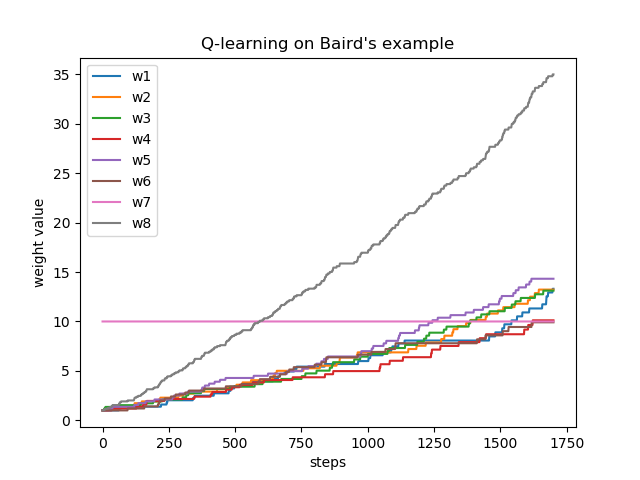
\includegraphics[scale=0.7]{q_learning_bairds}
  \end{center}

\end{enumerate}
\end{document}
